\glsresetall
How does knowing the evolutionary history of microbes affect our analysis of microbiological datasets? Depending on the research question, the common ancestry of microbes can be a source of confounding variation or can be a scaffolding used for inference. For example, when performing regression on traits the common ancestry is a source of dependence among observations, whereas when searching for clades with correlated abundances the common ancestry is the scaffolding for inference. The common ancestry of microbes and their genes is organized in trees – phylogenies – which can and should be incorporated into the analysis of microbial datasets.\par
While there has been a recent expansion of phylogenetically informed analytical tools, little guidance exists for which method best answers which biological questions. Here, we review methods for phylogeny-aware analyses of microbiome datasets, considerations for choosing the appropriate method, and challenges inherent in these methods.  We introduce a conceptual organization of these tools, breaking them down into phylogenetic comparative methods, ancestral state reconstruction, analysis of phylogenetic variables, and analysis of phylogenetic distances. Careful consideration of the research question and ecological and evolutionary assumptions will help researchers choose a phylogeny and appropriate methods to produce novel, accurate, and biologically informative insights.
\section{Introduction}
High-throughput sequencing yields information about microbial communities in quantities that outstrip our ability to make sense of it. Most microbial taxa have never been cultivated or experimentally characterized. For many, we have only sequence fragments, whole genome sequence data for a few distant relatives, and a tree capturing the microbes' evolutionary histories. How can we organize and analyze the deluge of information about uncharacterized microbes and their sequence fragments?\par
Two main tools for organizing the diversity of life are the taxonomy and the phylogeny. The taxonomy classifies a microbe based on a hierarchy of taxonomic names ranging from one of three domains (Bacteria, Archaea and Eukarya) to one of several million species. The phylogeny is an estimation of the microbes' evolutionary history which classifies every organism by a series of splits corresponding to estimated events in which a most recent common ancestor speciated to form two daughter species.\par
Microbial taxonomy and phylogeny may eventually be equivalent, with every clade in the phylogeny having a taxonomic name. However, contemporary taxonomic classification is coarse relative to the phylogeny; modern taxonomic labels categorize a small fraction of the branches in the phylogeny. For the time being, the phylogeny is a more detailed source of knowledge about the common ancestry of microbes.\par

Phylogenies are a tool to organize and understand the microbial world\cite{martiny_phylogenetic_microbiome} \cite{hug_tree_of_life}. Because related organisms tend to have similar characteristics, phylogenies can incorporate those characteristics into our analyses even if we can't measure them directly. Phylogenies are a scaffold to classify lineages and infer functional ecological traits, even for lineages that have not been classified taxonomically or physiologically. Microbial ecology can be accelerated by high-throughput classification and inferences made possible with phylogenies. Resource consumption \cite{tilman_resouce_competition}, habitat associations\cite{macarthur_bird_diversity} and species interactions\cite{may_ecosystem_stability}\cite{arditi_species_interact} are causes and consequences of traits, and using phylogenies to infer or implicitly work with traits may enhance our ability to manipulate microbial communities to impact human health \cite{hmp_structure}, biogeochemistry \cite{falkowski_microbial_chemistry}, and climate change \cite{bardgett_microbial_climate}.\par
How can a phylogeny assist analyses of microbiome data? Different research questions require different considerations about how to amend statistical analyses when considering a phylogeny. For example, studies testing associations between traits should consider the phylogeny as a source of dependence among observations, whereas studies looking for simpler ways of binning species should consider the phylogeny as a scaffolding for possible bins. There is a vast and growing literature on methods for analyzing phylogenetically-structured data, methods with subtle yet consequential differences in the questions they seek to answer. There is a need to simplify the diverse field into a set of conceptually distinct classes of methods and thereby provide a framework for instruction, comparison, and development of methods for analyzing phylogenetically-structured data.\par
In this review, we organize the field of phylogenetically-structured data analysis by discussing the major classes of methods. We first emphasize a fundamental issue in the field: the imperfection of estimated phylogenies. We then define four categories: (1) comparative methods, (2) ancestral state reconstruction and descendant trait imputation (3) variable analysis, and (4) phylogeny-aware distances (Table 1). Most statistical tools can be revisited for phylogeny-aware analyses, but the categories we cover capture the most commonly used and actively developed classes of methods. We discuss challenges of phylogenetically-aware analysis of microbiome data, including horizontal gene transfer (\gls{hgt}) and the choice of which genes to use when building phylogenies. By partitioning the literature into distinct conceptual classes of methods, we provide a common framework for the development and implementation of these important methods in microbiome data analysis.

\begin{table}[!ht]
        \caption[Comparison of different phylogentically aware methods.]{Comparison of different phylogentically aware methods. Different classes of methods for using the phylogeny in data analysis address different classes of questions. These methods can be summarized based on their use of given a dataset of abundance vectors, x, observed or imputed trait values, y, and the phylogeny, P. }

        \vspace{-0.25in}
        \begin{center}
                \begin{tabular}{|p{0.7in}|p{1.3in}|p{1.1in}|p{1.1in}|p{1.1in}|}
                        \hline
                        Class of Methods & Brief Description & Specific Example & General Formula & Highlighted Method \\
                        \hline
                        Comparative Methods &Find associations between traits, controlling for evolution on phylogeny & Is 16S \gls{rrna} gene copy number associated with growth rates in	vivo?& $y_{i}-g(Y)+\epsilon $
                        where

                        Conv $\left [ \epsilon  \right ]=f(P)$ & \gls{pgls}\cite{pgls}
                        Paired    \hspace{2cm}t-test\cite{martins_pcm} \\
                        \hline
                        Ancestral State Reconstruction & Impute trait values for historical
                        lineages in the phylogeny and use ancestral traits to impute trait
                        values for contemporary species & What is the best estimate of 16S \gls{rrna} gene copy number of
                        an \gls{otu} based on the 16S \gls{rrna} copy numbers of its relatives? & Infer features of $P|y $
                        Impute $y_{i,j}|y_{j}$ & PICRUSt\cite{picrust}  \\
                        \hline
                        Phylogenetic Variables & Use the phylogeny to construct	variables that are biologically
                        interpretable (for example, a clade's abundance) and simplify/summarize features in the
                        community & Which interior edges in P
                        separate taxa with different habitat associations? How does
                        Faith's phylogenetic diversity change with pH? &
                        Define variables:
                        $v_{i}= f_{i}(x,P)$  Analyse, interpret and combine $v_{i}$ & Diversity analyses
                        Taxonomic analyses Phylofactorization \cite{Washburne2017-up}
                        EdgePCA\cite{edgepca} Ph\gls{ilr}\cite{Silverman2016-he} \\
                        \hline
                        Phylogeny-Aware Distances & Use the phylogeny to construct distances between samples,
                        which can then be used to modify statistical tools for classification, regularized regression
                        and more & How different are two microbial communities? & Define distance
                        $d[x_{i},x_{j}]=K(x_{i},x_{j},P)$
                        Analyse and use to modify
                        various statistical methods & UniFrac\cite{unifrac, socolar_prey,
                          mccann_diversity, socolar_beta_diversity}\;
                        Inner product methods\cite{aitchison_statistics}, \cite{gloor_compositional_analysis}\\
                        \hline
                \end{tabular}
        \end{center}
        \label{tab:analysis3}
\end{table}

\section{Phylogenetic Inference}
The tree of life is not known; it is estimated, and accurate phylogenies improve accuracy of phylogenetically-structured data analysis. Microbial phylogenies are commonly estimated by collecting gene sequences, aligning sequences based on homologies, and using models of mutation to infer most-likely evolutionary histories. The estimated phylogeny can vary depending on which genes are sequenced, how sequence positions are aligned, which model of evolution is used, and the method for inferring histories. Errors in phylogenetic inference can propagate to errors in phylogenetically-structured data analysis. Here, we discuss the interplay between phylogenetic inference and phylogenetically-aware analyses; for a review of methods for phylogenetic inference, readers can consult focused reviews of that topic \cite{molecular_evolution, molecular_phylogenetics}.\par
One can construct a phylogeny for any gene, and different genes will vary in the number of species containing the gene, the accuracy of the phylogeny, and phylogenetic signal of a set of traits. The 16S \gls{rrna} gene is commonly used for phylogenetic inference in Bacteria and Archaea, but one could also construct a phylogeny for other genes such as beta lactamases and their relatives, yielding a phylogeny with edges along which antibiotic resistance traits arose \cite{molecular_evolution}. Microbial Eukaryotes likewise have many genes which can be used for phylogenetic inference, the 18S \gls{rrna} gene being most commonly used\cite{hillis_ribosome}. \par
The genes chosen for phylogenetic inference ultimately determine the set of traits correlated with the phylogeny. Bacterial genome trees generally correlate with the 16S \gls{rrna} gene (16S)-derived phylogenies\cite{snel_genome_phylogeny}, but the correlation between a 16S tree and gene content varies over lineages and phylogenetic depths\cite{zaneveld_ribosome}. \gls{hgt} disrupts the correlation between 16S trees and gene content by allowing bacteria with distant 16S genes to share common and consequential traits, such as pathogenicity islands and antibiotic resistance genes\cite{hall_lactamase,prokaryotic_evolution}. Moreover, the 16S sequence has multiple variable regions, and can vary among multiple copies within the same genome, complicating phylogenetic inference\cite{variability_16s}. More complicated scenarios, such as when epistasis underlies a functional ecological trait and one of the epistatic genes can be horizontally transmitted, prohibit a clear prescription for which gene's tree should be used for phylogenetic inference.\par
Different methods for analyzing phylogenetically-structured data use different features of the phylogeny. Distances and phylogenetic comparative methods which aggregate information over many branches in the phylogeny are more robust to errors in phylogenetic inference\cite{weighted_unifrac,robust_phylogenetic_regression} . Methods which rely on a few branches are more sensitive to errors in phylogenetic inference \cite{riesenfel_phylogeny}. For methods relying on a few internal nodes or branches, the uncertainty in phylogenetic inference – particularly the bootstrap support for the monophyly of critical branches\cite{felsenstein_confidence} – may be an important measure of uncertainty to incorporate into downstream data analysis. Where monophyly is crucial, researchers can collapse resolved nodes into polytomies to improve the bootstrap support across the whole tree. A more certain yet coarse-grained phylogeny may be preferable to a less certain yet fully resolved phylogeny.  Incorporating phylogenetic information has the capacity of drawing hypotheses on organisms never observed before.  While the vast majority of microbial life on the planet is not cultureable,phylogenetic analyses allow us to extrapolate and infer characteristics about unknown organisms based on closely related, cultureable organisms.
\section{Phylogenetic Comparative Methods}
Phylogenetic comparative methods (\gls{pcm}s) are used when comparing multiple traits across organisms. Closely related organisms often have similar traits due to inheritance from a common ancestor; such dependence of traits across organisms can affect tests of trait:trait and trait:habitat associations. \par
For example, we may find an association between 16S copy number (trait) and pH preference (habitat) through a correlation between 16S copy number and a measure of pH preference across 1,000 species of microbes (figure \ref{fig1a}a). Such an association could yield a false positive result if the taxa consist of a set of closely related of Acidobacteria with low 16S copy number and low pH preference, and a set of closely related Fusobacteria with high 16S copy number and a high pH preference\cite{variability_16s}. Intuitively, the phylogenetic signal of these traits reduces our sample size because the observed traits represent samples from two lineages, not 1,000 independent species. More rigorously, the phylogeny affects the covariance structure of residuals under null models of trait evolution. Robust tests of trait-associations are done using \gls{pcm}s\cite{grafen_regression} \cite{martins_pcm} (figure \ref{fig1a}b). \par
How does one account for dependence among trait observations? Generalized least squares can control for dependence among observations when performing regression. In generalized least squares, the residuals have an expected covariance under a null model and the covariance matrix is incorporated into least-squares calculations. For regression analyses, such as looking for associations between 16S copy number and habitat preference, phylogenetic generalized least squares\cite{blomberg_pgls} (\gls{pgls}; figure \ref{fig1a}) is a popular method using generalized least squares to correct for the expected covariance of residuals under null models of trait evolution along the branches of the phylogeny \cite{pagel_evolution}. \par
To implement \gls{pgls}, one first estimates the nature and magnitude of phylogenetic signal in the response variable. Pagel's $\lambda$ \cite{pagel_evolution} or Blomberg et al.'s $\kappa$ \cite{blomberg_test} are commonly used test statistics for phylogenetic signal. The phylogenetic signals from Pagel's $\lambda$, Blomberg's $\kappa$, or other metrics define covariance matrices of the residuals which can be used in generalized least squares (figure \ref{fig1a}b). For more complicated models of evolution, one can jointly estimate the parameters for the evolutionary model and the regression coefficients \cite{lavin_morphometrics}.\par
\gls{pcm}s extend to many statistical tests. Testing whether the volume of bacterial spores is smaller than the volume of daughter cells would involve a paired t-test, absent phylogenetic signal. A phylogenetic paired t-test\cite{lindenfors_test} was developed to account for phylogenetic signal in such tests. There are many models of trait evolution, metrics of phylogenetic signal, and methods to control for phylogenetic signal when comparing traits. A recent scholarly edition of modern \gls{pcm}s provides a review of the field and directions of current research\cite{pgls}.\par
\begin{figure}[H]
        \centering
        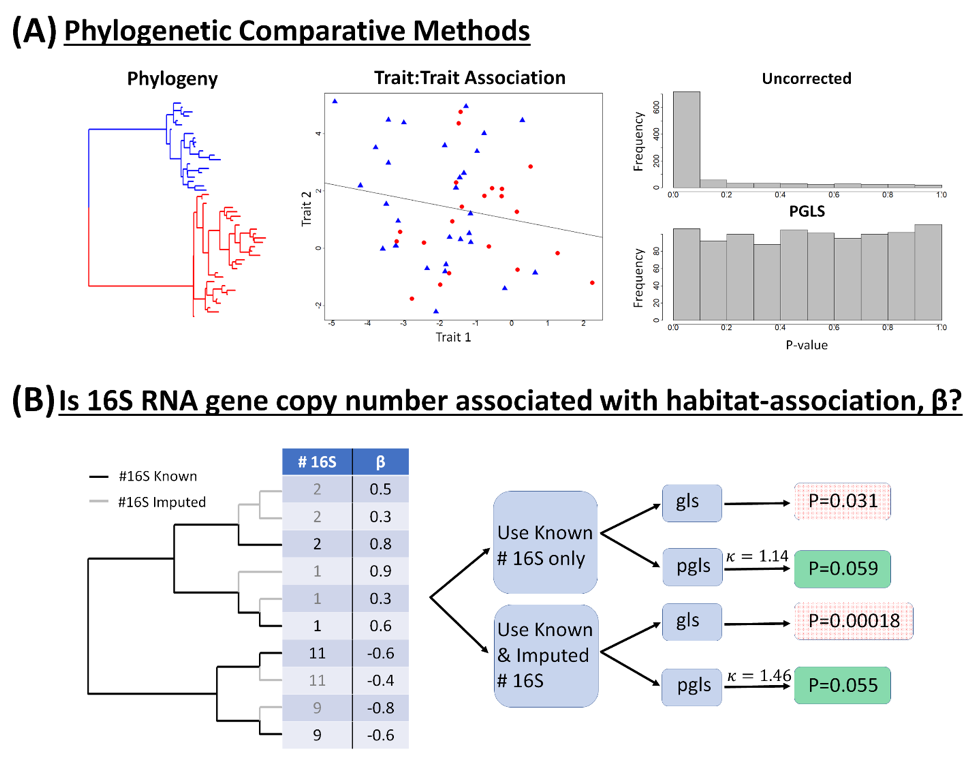
\includegraphics[width=1\textwidth]{ch1/figure1.png}
        \caption[Advantages of using phylogenetic comparative methods.]
        {Advantages of using phylogenetic comparative methods. Phylogenetic comparative methods control for the statistical dependence among traits resulting from evolution of traits along the phylogenetic tree. (A) An exaggerated phylogeny with two distantly related clades. If trait evolution is simulated as a random walk on the phylogeny, the two distantly related clades will drive covariances between traits. Failing to correct for the effects of random trait evolution can lead to a high false-positive rate. Methods such as phylogenetic generalized least squares (\gls{pgls}) correct for the residual covariance expected under random trait evolution and produce more accurate statistical tests of association. (B) \gls{pgls} should be used when testing associations between traits, even trait quantities such as regression coefficients from abundance~meta-data associations. To implement \gls{pgls}, a model of trait evolution needs to be assumed or estimated. Here, we estimate Blomberg's $\kappa$. \gls{pgls} should be used regardless whether the traits used are known or imputed through ancestral state reconstruction.\index{SanDiego}}
        \label{fig1a}
\end{figure}
\gls{pcm}s are not commonly used in microbiome studies, although a recent study\cite{bradley_phylogeny_correction} has employed \gls{pcm}s to identify genes associated with colonization of the human gut (trait:habitat). Failure to correct for phylogenetic dependence in tests of trait:trait and trait:habitat association can yield a high false-positive rate (figure \ref{fig1a}). To amend this, we recommend researchers familiarize themselves with and utilize \gls{pcm}s. Many methods can be implemented through the R packages \cite{ape} , phangorn \cite{phangorn}, phytools\cite{phytools}, picante\cite{picante}, caper \cite{caper}, Geiger \cite{geiger}, and phylglm\cite{phylglm}. In the supplemental online tutorial (https://knightlab-analyses.github.io/phylogenetic-tutorials/), we illustrate how these packages can be used to simulate trait evolution and test associations between traits. We also illustrate the sensitivity of these methods to \gls{hgt}.
\section{Ancestral State Reconstruction}
Estimating, or reconstructing, ancestral trait values assists imputation of traits in uncharacterized species and identification of historical lineages along which major trait differences arose. In studies of microorganisms, ancestral state reconstruction is commonly used to estimate genetic and metabolic profiles of extant communities using a set of reference genomes. In microbiome studies, this is commonly performed using PICRUSt\cite{picrust}, which uses pre-calculated ancestral state reconstructions to impute trait values, such as genes encoding glycoside hydrolase activity, for taxa whose traits are unknown.\par
PICRUSt operates on a phylogenetic tree, constructed from 16S sequences, connecting various sequenced genomes and environmental sequences. First, trait information observed in the sequenced genomes is used to infer ancestral trait profiles. Ancestral profiles are then used to predict the profiles of each organism in an environmental sample. An input sample's predicted metagenomic profile is then estimated by adding the product of \gls{otu} abundances in the sample and their corresponding profiles. Because this method relies strongly on the reference database, and the available sequenced genomes, it underperforms in environments where few or no genome data is known. Conversely, PICRUSt was able to predict the profiles of whole genome shotgun human fecal samples with a Spearman $R^2$ of $>$ 0.9 \cite{picrust}, suggesting that the microbial phylogeny is high predictive of microbial genome content.\par
The methodology underlying ancestral state reconstruction are very similar to phylogenetic comparative methods, as both require considering models of evolution \cite{ancestral_character_states}. Three main types of algorithms are used to connect the tree, traits, a model of evolution, and estimates of ancestral states given the model of evolution: maximum parsimony, maximum likelihood and Bayesian inference\cite{ancestral_character_states}. Maximum parsimony reconstructs ancestral states by minimizing the number of trait changes between the ancestor and the present descendants. This approach assumes that trait changes are slow, and does not account for scenarios involving rapid evolution. In addition, maximum parsimony treats all branches the same and minimizes the number of changes on each branch; this can be problematic, particularly if not all of the species have been observed \cite{ancestral_reconstruction}. Maximum likelihood and Bayesian inference improve on maximum parsimony by incorporating explicit models of evolution – such as a Brownian motion model of trait evolution along the tree - into the estimation of ancestral states. Rather than simply assuming that changes are rare, these methods can account for some changes occurring more frequently than others—for example, assuming synonymous substitutions are more frequent than non-synonymous substitutions—and fit parameters to these models given an estimated phylogeny.  However, maximum likelihood will often underestimate the number of changes within a single branch and can generate suboptimal results, particularly if the rate of evolution changes across the phylogeny \cite{simulation_comparison}. Bayesian approaches can compute evolutionary parameters across a deep sampling of possible evolutionary trees and evaluating more complex models of evolution that account for non-uniform rates of evolution. While Bayesian methods can generate more accurate results than maximum parsimony or maximum likelihood, they can be computationally expensive with large numbers of species.  Consequently, PICRUSt estimates microbial ancestral states using maximum parsimony or maximum likelihood. \par
As for phylogenetic comparative methods, estimates of ancestral states can be quickly confounded by \gls{hgt} (see supplemental online tutorial), and thus applications of these methods to microbial datasets should be performed with consideration of the observed rates of transfer for the gene families of interest.
\section{Analysis of phylogenetic variables}
While points on the Earth's surface can be located with three Cartesian (xyz) coordinates, we naturally describe locations using two spherical coordinates (latitude and longitude). A phylogeny, like a sphere, defines the map of biological data and suggests natural coordinates. Phylogenetic variables are used to reduce the dimension of community ecological data, simplify calculations of distances, and describe meaningful features and directions of change in communities (figure \ref{figa2}).
We coin the term “phylogenetic variables” to describe variables constructed using features in the phylogeny to aggregate, contrast, and summarize data of species in the phylogenetic tree (figure \ref{figa2}). Variables and distances are related, but contain distinct information: saying the city is east doesn't indicate how far it is, and saying a city is 80 kilometers away doesn't indicate which direction it is. Directions are described through phylogenetic variables (figure \ref{figa2}A), and the magnitude of changes is measured through distances (figure \ref{figa2}B). Phylogenetic variables include diversity metrics, taxonomic abundances, differences of abundance along all edges \cite{picante}, differences of abundances between clades (figures \ref{figa2}A, \ref{figa2}C, \ref{figa2}D) \cite{Washburne2017-up} \cite{Silverman2016-he}, and more. \par
\begin{figure}[H]
        \centering
        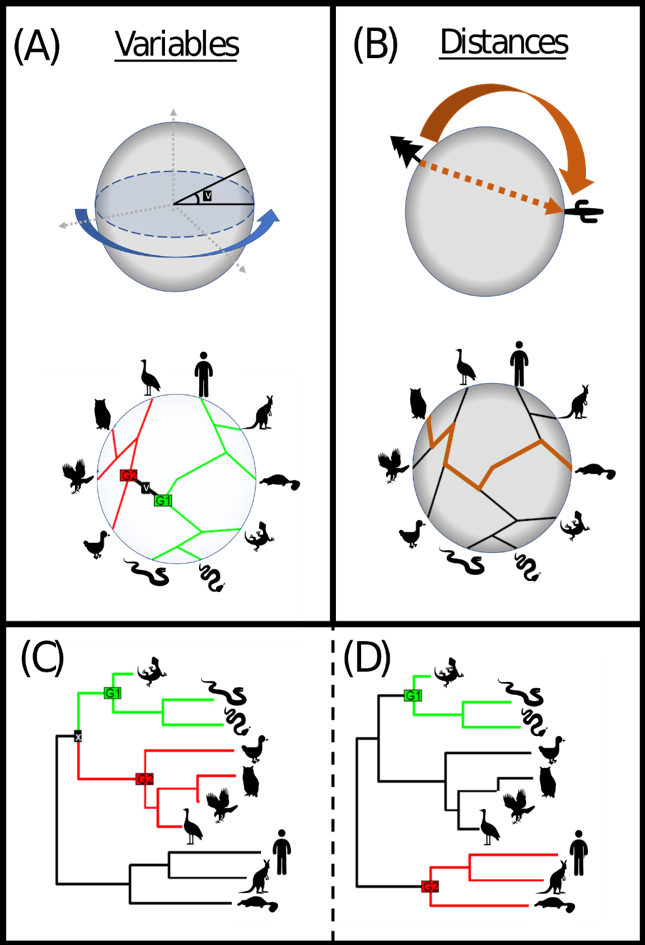
\includegraphics[width=0.7\textwidth]{ch1/figure2.png}
        \caption[A comparison between phylogenetic variable analysis and phylogenetic distances.]
        {A comparison between phylogenetic variable analysis and phylogenetic distances. Phylogenies define the geometry of community ecological data, much like a sphere defines the geometry of GPS data. (A) Changing variables can allow more natural descriptions of complex topologies. A spherical Earth motivates spherical coordinates. Phylogenetic variables use the tree as a scaffolding for constructing coordinates corresponding to phylogenetic features. Phylofactorization constructs coordinates contrasting groups, G1 and G2, separated by edges where traits such as flight arose. (B) A default path between two points is a straight line, but a more meaningful path on a sphere is “as the crow flies”. Likewise, phylogeny-aware distances such as UniFrac define evolutionary paths and their distances between one community to another. (C) Ph\gls{ilr} constructs coordinates contrasting sister clades. (D) The space of possible phylogenetic variables and distances is infinitely large. Researchers should consider the biological interpretability of novel variables and distances, and their ability to inform future studies.\index{SanDiego1}}
        \label{figa2}
\end{figure}
Phylogenetic variables simplify microbiome datasets by reducing the dimension of the data to a few variables carrying biological information. If a few monophyletic clades explain the majority of a microbiome dataset's variance along an environmental gradient, then there may be traits, shared among members of each clade, which are important determinants of abundance along the environmental gradient and underlie the observed community compositional changes.
The set of possible phylogenetic variables is infinitely large. Consequently, researchers must be deliberate in their choice of novel phylogenetic variables – what are important directions of change that carry implications for further research? Community changes along the direction of a phylogenetic variable, such as alpha diversity, does not necessarily convey useful biological information or immediate implications for future study design. Two common challenges in the analysis of phylogenetic variables can help guide the choice and development of phylogenetic variables: statistical dependence and biological interpretability.
Statistical independence, or well-characterized dependence, facilitates robust multivariate statistics and multiple comparisons corrections. For instance, when testing associations between species' abundances and environmental meta-data, and repeating the process for genera, families, orders, classes, and phyla, the variables analyzed have a nested dependence: if one taxon increases in abundance, all else being equal it will increase the abundance of all higher taxonomic groups in which it is found. For another example, if every sequence discovered is novel, the Shannon diversity of n sequences and n species will be H=log(n) and the species richness and evenness across samples will be correlated. Failing to account for the dependence among phylogenetic variables can increase error rates when performing multiple hypothesis tests.\par
Phylogenetic variables with a clear biological interpretation can carry implications for future study design and biological theory development. Changes in the abundance of a monophyletic clade may suggest a heritable trait driving changes in abundance; future experiments can focus on the clade to search for possible functional ecological traits. In macroscopic ecology, theoretical arguments justify the utility of various diversity metrics as proxies for extinction rates, island-biogeographic processes, ecosystem stability, and conservation goals\cite{socolar_prey,socolar_beta_diversity,mccann_diversity}.  Theoretical justification and interpretation of phylogenetic variables connects the analysis of phylogenetic variables (e.g. associations between diversity and meta-data) with experimental design and biological theory.\par
Two recently developed methods —Ph\gls{ilr} \cite{Silverman2016-he} and phylofactorization \cite{Washburne2017-up} illustrate the challenges of phylogenetic variables analysis. Motivated by the compositional nature of sequence-count data \cite{aitchison_statistics} \cite{gloor_compositional_analysis}, both methods construct variables through average log-ratios of abundances between two clades in the phylogeny.  Ph\gls{ilr} variables measure the difference between sister clades (figure \ref{figa2}C), and phylofactorization iteratively constructs variables measuring the difference between clades separated by edges in the tree (such as those in figure \ref{figa2}A,D).\par
Changes in a Ph\gls{ilr} coordinate may indicate a trait differentiating sister clades, whereas changes in coordinates from phylofactorization may indicate a trait arose along the identified edge. In both methods, significant associations between phylogenetic variables and meta-data motivate future work comparing genomes of two clades to search for functional traits. Ph\gls{ilr} motivates comparison of sister clades (e.g. placental mammals to marsupials, or birds to crocodiles), whereas phylofactorization implicates comparison of clades separated by edges (e.g. birds to non-birds). In the supplementary tutorial, we illustrate these two methods for phylogenetic variables analysis, show how to construct these variables, compare them to EdgePCA, analyze a simulated dataset where \gls{rrna} gene copy number drives associations with disturbance frequency in soils\cite{rrna_operon}, and interpret the results.
The goal of analyzing phylogenetic variables is to identify meaningful directions of change in microbiome data. Much like how principal components analysis can identify major directions/axes of variation in a dataset, phylogenetic variables can identify directions of change in microbiome data which explain variance in community composition and have implications for extinction risk, which organisms to cultivate, which genomes to search, and more.
\section{Using Phylogeny-Aware Distances }
Quantifying the dissimilarity between different species and between different communities comprising these species can facilitate accurate classification of meta-data (such as whether a patient has a disease), clustering of samples, and inferences of community function. Trees in forests sequester carbon in wood, whereas grasses do not. Consequently, measures of distance between communities containing trees from communities containing grasses may be indicative of differences in the ecosystem physiology of forests and grasslands. For the microbial world, traits driving ecosystem function are often unknown, yet accurate classification of disease states can have major consequences for human health and, where traits analogous to woody biomass underlie habitat associations, incorporating the phylogeny into distance measures can aid classification (figure \ref{figa3}). \par
One of the most widely used methods for phylogeny-aware analysis of microbiome data is the analysis of UniFrac distances between samples\cite{unifrac}. The UniFrac distance was motivated as a more biologically meaningful distance between communities than standard Euclidean and Bray-Curtis distances. The intuition behind UniFrac, and most phylogeny-aware distances, is that communities containing more phylogenetically distinct species are more different than communities with more closely related species. Incorporating phylogenetic distances along which functional changes occur may better quantify functional differences between communities.\par
Many extensions of Unifrac have been explored with the aim of controlling statistical artifacts in count data and tuning the importance of abundance in UniFrac distances. If counts are randomly distributed among species, clades with more species will have higher variances in total counts and thus have greater impact on UniFrac distances than clades with fewer species. To remedy this effect, VAW-UniFrac\cite{vaw_unifrac} stabilizes the variance of UniFrac distances. VAW-UniFrac was extended by the Generalized Unifrac Distance \cite{generalized_unifrac}, which contains a tunable parameter to increase/decrease the importance of abundance in the distances between communities. \par
\begin{figure}[H]
        \centering
        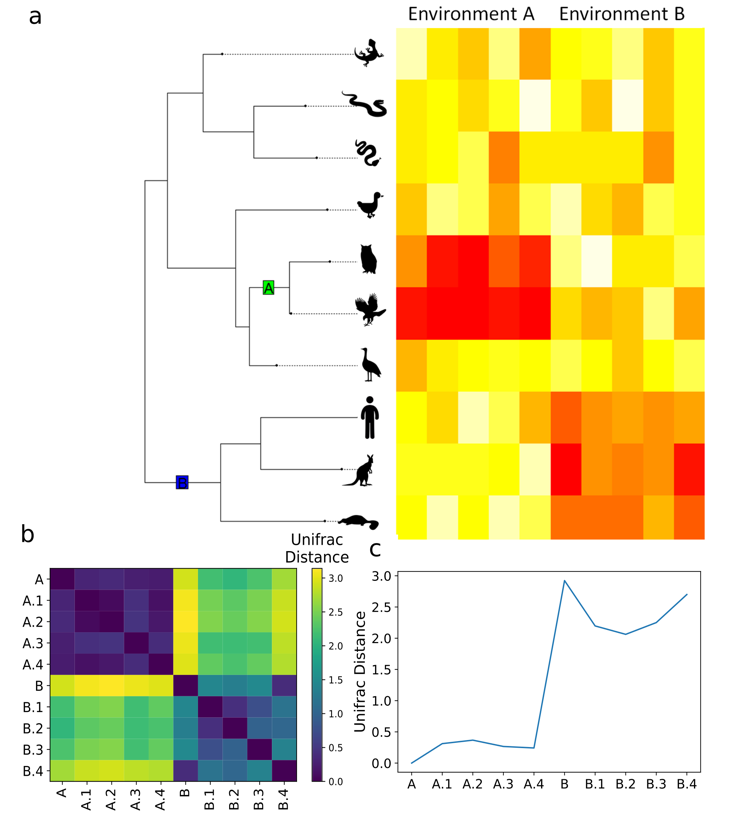
\includegraphics[width=0.7\textwidth]{ch1/figure3.png}
        \caption[A demonstration of how to interpret Unifrac distances.]
        {A demonstration of how to interpret Unifrac distances.(a) A heatmap of species abundances with red indicating high abundance and yellow indicating low abundance across different environments.  The evolutionary history is represented by the phylogenetic tree, and the main differences between Environment A and Environment B are being driven by the abundances in clade A and clade B. (b) While variables contain information for each sample, distances relate two samples. Plotted are the pairwise Unifrac distances between the samples; distances between samples from Environments A and samples from Environment B are larger compared to distances between samples from Environment A or distances between samples from Environment B. (c) The Unifrac distance between a sample from the Environment A to all other samples illustrates how distances can be useful for sample-site classification. Phylogeny-aware distances can relate to functional distances by capturing flow of abundances through edges along which traits arose.\index{SanDiego3}}
        \label{figa3}
\end{figure}

UniFrac distances are not the only possible phylogenetically-informed distances.  There have been a number of different distance metrics such as Sorensens' index, Rao's D and Rao's H that have been proposed alternative methods to incorporate evolutionary information \cite{Silverman2016-he}.  Furthermore, standard statistical techniques such linear regression can be augmented to penalize differences between close relatives\cite{phylogenetic_cca,purdom,fukuyama_perturbation}.The phylogeny is a scaffold for many variables, and can serve as the basis for many useful distance metrics. Which distance(s), of the possible distances, are of interest to a given microbiologist? \par
We suggest two main goals in the construction of phylogeny-aware distances: improving sample-site classification/visualization and providing meaningful interpretations of community differences. \par
If sample-site visualization is the goal of an experiment, a researcher may be inclined to search through a space of possible distances until finding one that looks the best, irrespective of the biological interpretability of the distance. Otherwise, searching too many distances risks dredging the data and presenting statistically significant patterns which were obtained by testing multiple candidates without proper corrections for multiple hypothesis tests performed. Correcting for such multiple tests will face the same challenges of unclear dependence among tests that arise in the analysis of multiple phylogenetic variables.
While many existing distances can successfully classify samples across a range of site categories and clinical variables, the biological implications of discovered differences are often unclear. Does a larger distance indicate greater difficulty in bioremediation of one community into another? Does a larger distance imply a larger difference in ecosystem function or patient morbidity? What follow-up experiments should one conduct to better understand the biochemical and microbiological causes of community differences, given a large UniFrac distance?\par
Construction of new phylogeny-aware distances and their use in modified statistical methods should consider the performance gains relative to existing methods and whether they provide a new interpretation of discovered differences. Careful justification of new distances can improve the biological interpretation of results. For instance, macroscopic ecologists debate how beta diversity can be used for conservation\cite{socolar_beta_diversity}. Such discussions can improve the interpretation of existing and newly developed phylogeny-aware distances and help researchers understand any implications of high or low distances between communities. In addition, a high quality tree is critical for revealing ecologically relevant patterns \cite{fast_unifrac}.  As with phylogenetic comparative methods and phylogenetic variables, phylogeny-aware distances benefit from explicit consideration of ecological and evolutionary models to aid the biological interpretation of their results.
\section{Challenges of phylogenetic analysis}
There are challenges to phylogenetically-structured data analysis, including \gls{hgt}, the choice of which gene tree to use, the sensitivity to errors in phylogenetic inference, and the explicit consideration of ecological and evolutionary models.\par
\gls{hgt} between microbial genomes complicates the evolutionary story of vertical transmission captured in a phylogenetic tree \cite{gogarten_hgt}. \gls{hgt} raises the question of which phylogeny to use and how informative the phylogeny is for the research question. For phylogenetic comparative methods, \gls{hgt} can lead to improper corrections and poorly calibrated statistical tests (illustrated in supplement). \gls{hgt} of a major trait driving variation in the data can reduce the appropriateness of the phylogenetic variables or distances being used.\par
It is favorable to choose gene families that are insensitive to \gls{hgt} for inferring phylogenies. Studies have evaluated the chance of \gls{hgt} based on functional and ecological features\cite{gogarten_hgt, complexity_hypothesis}, providing guidelines for this task. Perhaps there is no gene absolutely \gls{hgt}-free throughout the tree of life, including 16S \cite{kitahara_hgt}. Including multiple genes in phylogenetic inference can minimize the negative impact of \gls{hgt} \cite{phylophlan}, and reveal genes influenced by \gls{hgt} within the selected range of taxa\cite{purdom}. Computational tools are available for assessing the probability of putative \gls{hgt} events based on species/gene tree reconciliation\cite{Washburne2017-up}. Exploration of genomic context, sequence signature and atypical homology search results also help tracking \gls{hgt}s\cite{ravenhall_hgt}. \par
\gls{hgt} does not invalidate phylogeny-aware analyses of microbiome data. \gls{hgt} of functional traits could be hypothesized through phylogeny-aware analyses by strong effects with little phylogenetic signal \cite{lozupone_species_divergence}. If phylofactorization identifies an unusually large number of tips of the tree associated with antibiotic exposure, \gls{hgt} may be driving variation in the data and can be further tested by comparison of genomes among the phylogenetic factors identified. Nonetheless, \gls{hgt} requires consideration when analyzing phylogenetically-structured data. The sensitivity of many methods to the horizontal transfer of functional traits is currently understudied. The combination of \gls{hgt} and the existence of different phylogenies for each gene motivates careful justification of which genes to use to make phylogenies.
Finally, all methods face the challenge of being interpretable and advancing our knowledge of microbiological systems. To that end, new methods should explicitly consider ecological and evolutionary models for how traits evolve and drive patterns in the data. One study simulated trait evolution on a tree and compared \gls{pgls} with phylogenetic eigenvector regression methods\cite{phylogenetic_eigenvector}, which use eigenvectors from phylogenetic distance matrices as explanatory variables and do not correspond to a clear evolutionary model. The study found that \gls{pgls} produced more reliable and better-calibrated statistical results\cite{phylogenetic_eigenvector}. Considering evolutionary and population genetic models in method development promotes accurate understanding of the assumptions under which a phylogeny-aware analysis performs well and interpretation of findings in terms of the biological processes at play\cite{comparative_methods_fix}. \par
As more methods are developed, researchers should be aware of the tradeoffs between machine learning and human understanding: the former may produce more accurate predictions in the short term, whereas the latter produces theory that can generate more accurate and generalizable predictions in the long term.\par
\section{Discussion}
The common ancestry of microorganisms can be a source of confounding variation in our data, or a scaffolding on which we make inferences. There are many existing and emerging methods for analyzing microbiome datasets in light of evolution, and choosing the right method requires precise statements of the research question (Table 1).\par
First, decide which tree to use. Commonly, microbiome studies use the 16S tree for Bacteria and Archaea and the 18S tree for microbial eukaryotes, but there is a phylogeny for every gene and some questions are better analyzed with trees from other genes. The phylogeny obtained will be an estimate, and uncertainty in phylogenetic inference can translate to uncertainty in downstream phylogenetically-structured data analysis.\par
If the research question uses a trait as a response variable, the phylogeny may be a source of confounding variation. Phylogenetic comparative methods, such as \gls{pgls}, correct for dependence among traits one expects under null models of evolution along the tree.\par
If the research question is seeking historical trait values, or edges along which major trait differences arose, ancestral state construction is needed. If testing associations between imputed traits, researchers need to combine ancestral state reconstruction for imputation of missing traits with phylogenetic comparative methods which correct for confounding variation. \par
If the research question aims to simplify patterns of community composition, the phylogeny is a scaffolding that can be used to produce biologically informative variables and directions of change. The choice of variables should be made according to their ability to capture features in data, their statistical dependence, and their biological interpretation.\par
If the research question is to differentiate microbial samples, the phylogeny can define distances between samples. By re-defining distances, the phylogeny can be used to modify virtually any statistical method, but the choice of which distance to use should be based on the research goals of sample-site classification or biological interpretation of differences.\par
Phylogenetic analysis of microbiome data can allow researchers to categorize unclassified microorganisms, test evolutionary hypotheses about trait associations or traits driving habitat associations, and better understand how microbial communities differ and how they change over time, space, and treatments. There are several classes of methods for analyzing microbiome data “in light of evolution”. Careful consideration of the research question and the allowable ecological and evolutionary assumptions enables researchers to identify existing methods or produce novel methods that address their research question and produce novel, accurate, and biologically informative insights. The deluge of information about microbial sequences is producing phylogenetically-structured data which, given the right tools, can accelerate our understanding of microbial community structure and function.

\section{Acknowledgements}
J.T.M. was funded by NSF GRFP DGE-1144086. A.D.W. received support from Duke University Biology Department’s provision of start-up funds for D. Nemergut (deceased) and the Defense Advanced Research Projects Agency (DARPA) grant D16AP0013. This paper is published in the spirit of D. Nemergut’s contagious love of science.

Chapter 1, in full, is a reprint of the material as it appears in
``Methods for phylogenetic analysis of microbiome data''
Alex D. Washburne, James T. Morton, Jon Sanders, Daniel McDonald,
Qiyun Zhu, Angela M. Oliverio, Rob Knight  \emph{Nature Microbiology} 3, 2018. The dissertation author was the primary investigator and co-first author of this paper.

